% \newpage
\section{\textbf{Modules:} the plasticity loss of critic network is predominant}
\label{Sec: Modules}

In this section, we aim to investigate \textbf{\textit{which module(s) of VRL agents suffer the most severe plasticity loss, and thus, are detrimental to efficient training}}.
Initially, by observing the differential trends in plasticity levels across modules with and without DA, we preliminarily pinpoint the critic's plasticity loss as the pivotal factor influencing training.
Subsequently, the decisive role of DA when using a frozen pre-trained encoder attests that encoder's plasticity loss isn't the primary bottleneck for sample inefficiency.
Finally, contrastive experiments with plasticity injection on actor and critic further corroborate that the critic's plasticity loss is the main culprit.

\textbf{Fraction of Active Units (FAU).}~~
Although the complete mechanisms underlying plasticity loss remain unclear, a reduction in the number of active units within the network has been identified as a principal factor contributing to this deterioration~\citep{understanding_plasticity, dormant_neuron, Enhancing_Generalization_Plasticity}.
Hence, the Fraction of Active Units (FAU) is widely used as a metric for measuring plasticity.
Specifically, the FAU for neurons located in module $\mathcal{M}$, denoted as $\Phi_\mathcal{M}$, is formally defined as:
\begin{align}
    \label{eqn:FAU}
    \Phi_\mathcal{M} = \frac{\sum_{n\in \mathcal{M}} \mathbf{1}(a_n(x) > 0)}{N},
\end{align}
where $a_n(x)$ represent the activation of neuron $n$ given the input $x$, and $N$ is the total number of neurons within module $\mathcal{M}$.
More discussion on plasticity measurement can be found in \Appendix~\ref{Appendix: Measurement Metrics of Plasticity}.

\textbf{Different FAU trends across modules reveal critic's plasticity loss as a hurdle for VRL training.} 
Within FAU as metric, we proceed to assess the plasticity disparities in the encoder, actor, and critic modules with and without DA.
We adopt the experimental setup from~\cite{DrQ-v2}, where the encoder is updated only based on the critic loss.
As shown in Figure~\ref{Fig:FAU} \textcolor{mylinkcolor}{(left)}, the integration of DA leads to a substantial leap in training performance.
Consistent with this uptrend in performance, DA elevates the critic's FAU to a level almost equivalent to an initialized network.
In contrast, both the encoder and actor's FAU exhibit similar trends regardless of DA's presence or absence.
This finding tentatively suggests that critic's plasticity loss is the bottleneck constraining training efficiency.

\begin{figure}[h]
  \centering
  \vspace{-1.1\baselineskip}
  % 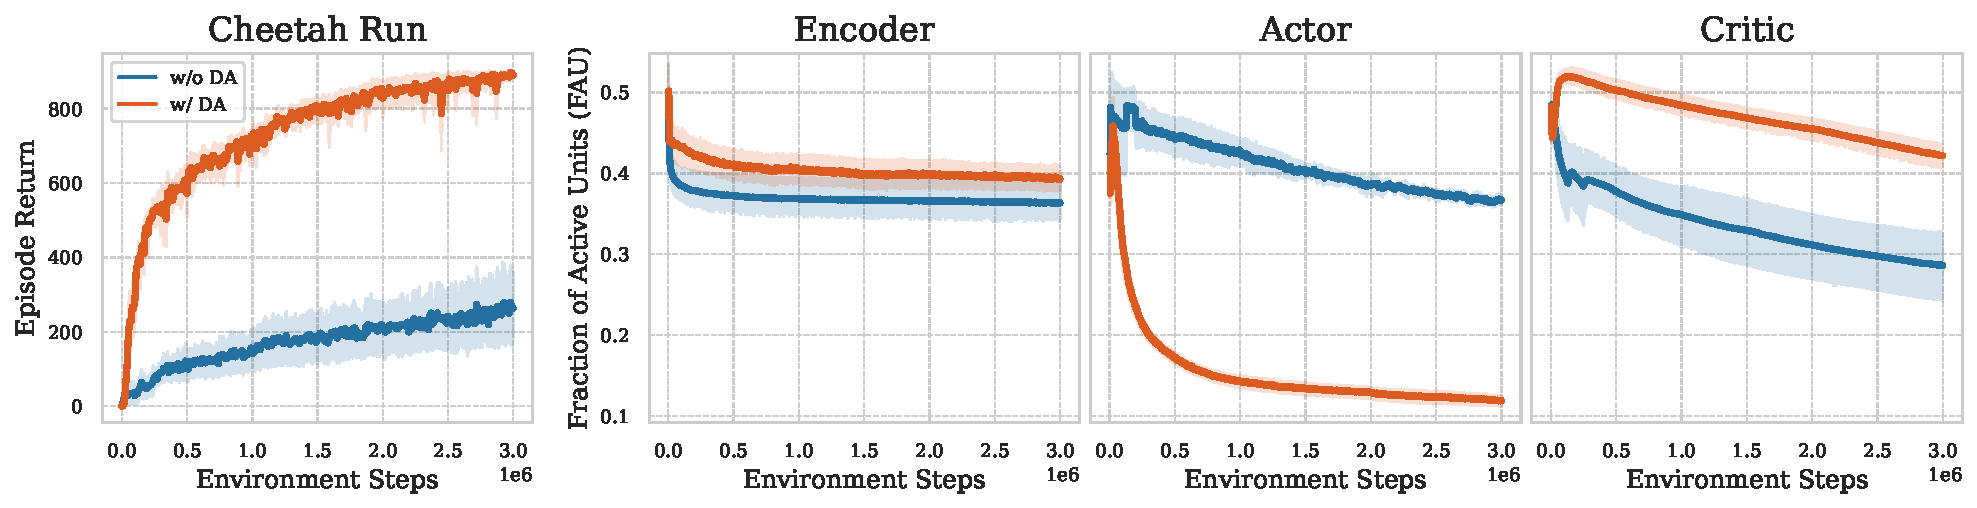
\includegraphics[width=\textwidth]{Figures/2Modules/FAU_cheetah_run.pdf}\\
  % \vspace{-0.3\baselineskip}
  % 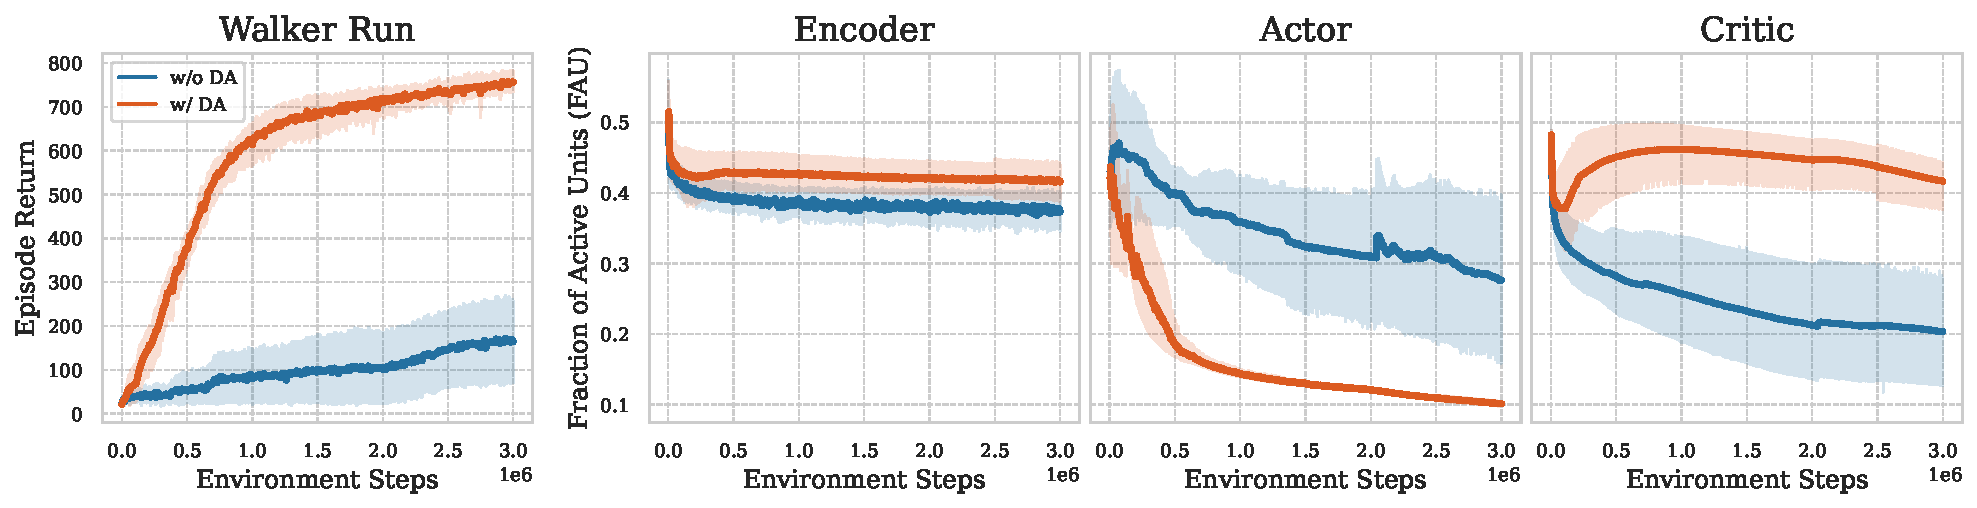
\includegraphics[width=\textwidth]{Figures/2Modules/FAU_walker_run.pdf}\\
  % \vspace{-0.3\baselineskip}
  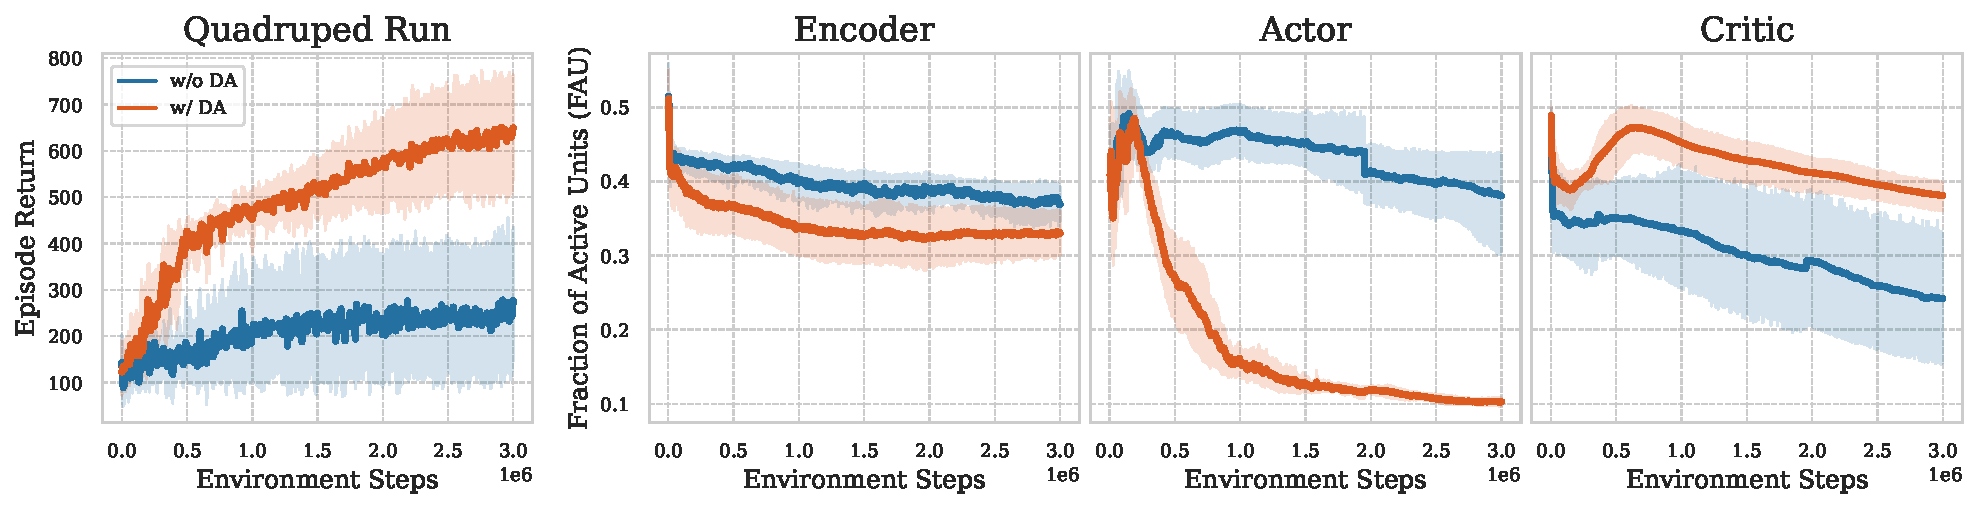
\includegraphics[width=\textwidth]{Figures/2Modules/FAU_quadruped_run.pdf} 
  \vspace{-2\baselineskip}
  \caption{Different FAU trends across modules throughout training. The plasticity of encoder and actor displays similar trends whether DA is employed or not. Conversely, integrating DA leads to a marked improvement in the critic's plasticity. Further comparative results are in \Appendix~\ref{Appendix: FAU trends}.}
  \label{Fig:FAU}
\end{figure}

\textbf{Is the sample inefficiency in VRL truly blamed on poor representation?}~~
Since VRL handles high-dimensional image observations rather than well-structured states, prior studies commonly attribute VRL's sample inefficiency to its inherent challenge of learning a compact representation. 

\begin{wrapfigure}[16]{r}{0.54\textwidth}
  \vspace{-\baselineskip}  
  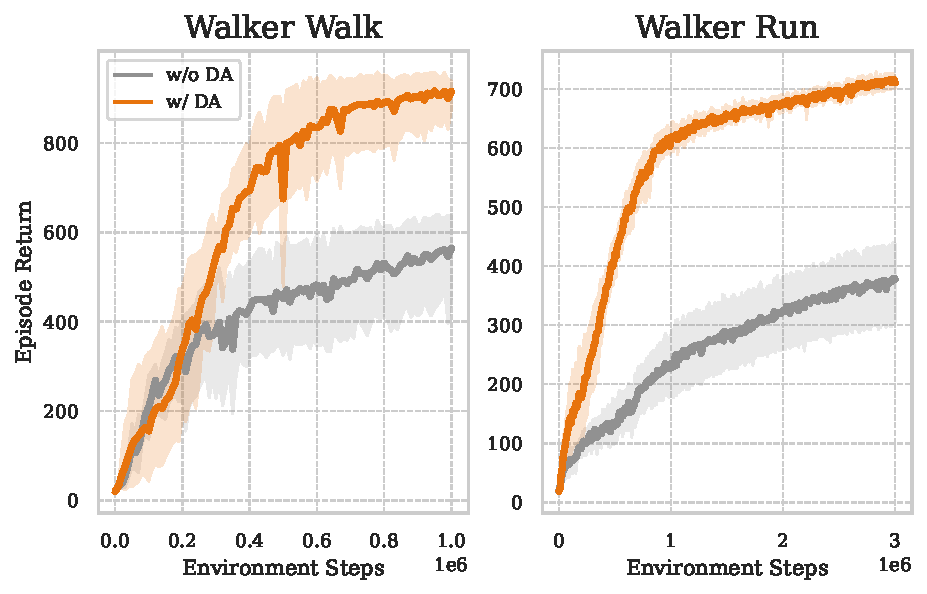
\includegraphics[width=0.54\textwidth]{Figures/2Modules/pre-trained_encoder.pdf}
  \vspace{-2\baselineskip}
  \caption{Learning curves of DrQ-v2 using a frozen ImageNet pre-trained encoder, with and without DA.}
  \label{fig:pretrain}
\end{wrapfigure}
We contest this assumption by conducting a simple experiment.
Instead of training the encoder from scratch, we employ an ImageNet pre-trained ResNet model as the agent's encoder and retain its parameters frozen throughout the training process.
The specific implementation adheres~\cite{yuan2022pre}, but employs the DA operation as in DrQ-v2.
Building on this setup, we compare the effects of employing DA against not using it on sample efficiency, thereby isolating and negating the potential influences from disparities in the encoder's representation capability on training.
As depicted in Figure~\ref{fig:pretrain}, the results illustrate that employing DA consistently surpasses scenarios without DA by a notable margin.
This significant gap sample inefficiency in VRL cannot be predominantly attributed to poor representation.
This pronounced disparity underscores two critical insights: first, the pivotal effectiveness of DA is not centered on enhancing representation; and second, sample inefficiency in VRL cannot be primarily ascribed to the insufficient representation.

% To discern the influence of DA on the encoder, we adopt an ImageNet pre-trained ResNet encoder, maintaining its parameters unchanged during RL training. We then compare the performance with and without DA. The comparative outcomes are depicted in Figure \ref{fig:pretrain}. Notably, the results illustrate that employing DA consistently surpasses scenarios without DA by a notable margin. This suggests that sample inefficiency in VRL cannot be predominantly attributed to poor representation.
% The results reveal that even when using a freeze pre-trained encoder during RL training, the performance with DA surpasses that without DA significantly.

\textbf{Plasticity Injection on Actor and Critic as a Diagnostic Tool.}~~
Having ruled out the encoder's influence, we next explore how the plasticity loss of actor and critic impact VRL's training efficiency.

\begin{wrapfigure}[19]{r}{0.5\textwidth}
  \vspace{-0.5\baselineskip}  
  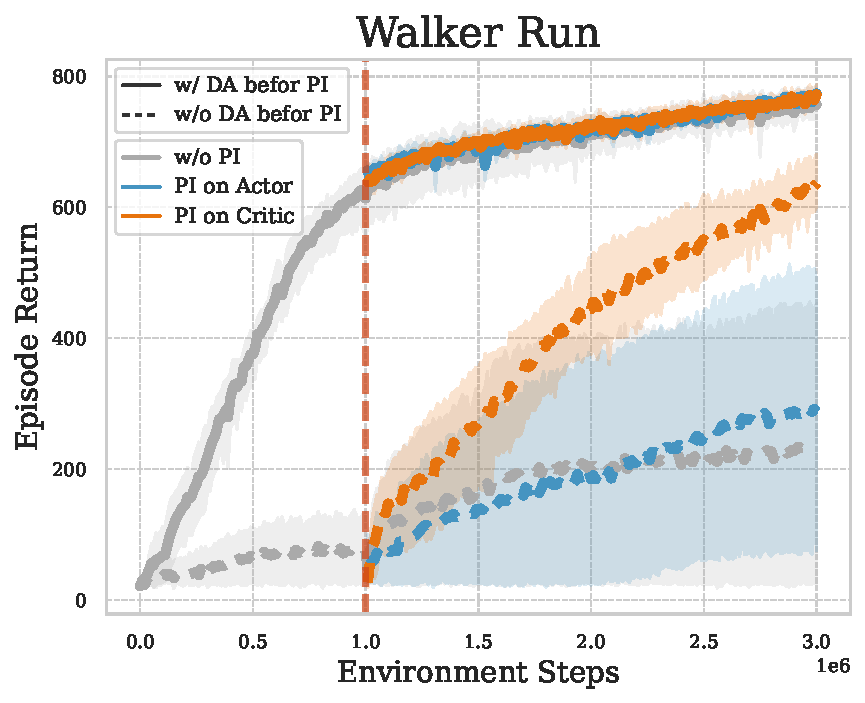
\includegraphics[width=0.5\textwidth]{Figures/2Modules/Injection_WR.pdf}
  \vspace{-1.5\baselineskip}
  \caption{Training curves of employing plasticity injection (PI) on actor or critic. For all cases, DA is applied after the given environment steps.}
  \label{fig:injection}
\end{wrapfigure}
To achieve this, we introduce plasticity injection as a diagnostic tool~\citep{Plasticity_Injection}.
Unlike Reset, which leads to a periodic momentary decrease in performance and induces an exploration effect~\citep{primacy_bias}, plasticity injection restores the module's plasticity to its initial level without altering other characteristics or compromising previously learned knowledge.
Therefore, plasticity injection allows us to investigate in isolation the impact on training after reintroducing sufficient plasticity to a certain module.
Should the training performance exhibit a marked enhancement relative to the baseline following plasticity injection into a particular module, it would suggest that this module had previously undergone catastrophic plasticity loss, thereby compromising the training efficacy.
We apply plasticity injection separately to the actor and critic when using and not using DA.
The results illustrated in Figure~\ref{fig:injection} and \Appendix~\ref{Appendix: Plasticity Injection} reveal the subsequent findings and insights:
\textcolor{mydarkgreen}{$\bullet$}~When employing DA, the application of plasticity injection to both the actor and critic does not modify the training performance. This suggests that DA alone is sufficient to maintain plasticity within the Walker Run task.
\textcolor{mydarkgreen}{$\bullet$}~Without using DA in the initial 1M steps, administering plasticity injection to the critic resulted in a significant performance improvement. This fully demonstrates that the critic's plasticity loss is the primary culprit behind VRL's sample inefficiency.
%While the injection on the critic significantly improves sample efficiency, particularly in the absence of data augmentation, the injection on the actor has no discernible impact.
